%==============================================================================
\chapter{GREY LITERATURE}\label{grey_literature}
%==============================================================================

Before beginning to develop the solution itself, it would be extremely beneficial to conduct a systematic review of the grey literature to map and assess existing tools and solutions that already address the issue of managing outreach activities in the context of \acp{HEI}. This research will ultimately result in a software product. Two authors did the review. Although the two term papers were prepared independently, as was already indicated, the artifacts produced to support the study were produced jointly.

The systematic review of the gray literature is described in this chapter. Additionally, data gathered during the study that is pertinent to the creation of the target product will be presented. In addition to a thorough examination and comparison of the chosen tools, the protocol established to conduct the evaluation will be covered, citing details such research questions, inclusion and exclusion criteria, extracted data, and search strings.

In this manner, the chapter is structured: Introduced in the \Cref{sec:gl-background} are words and ideas utilized in the study. The technique outlined by the authors will be presented in \Cref{sec:gl-planning}. The methods used in the study and the information gathered to address the research questions will be explained in the section on reporting \Cref{sec:gl-reporting}, while the section on validity \Cref{sec:gl-validity} highlights risks to the study's validity. The systematic review is concluded by \Cref{sec:gl-considerations}.

\section{Background}\label{sec:gl-background}

The following definition of grey literature comes from \citeonline{garousi2019guidelines}:
\begin{citacao}
  <grey literature> is produced at all levels of government, academia, business, and industry in print and electronic formats, but is not controlled by commercial publishers, or that is, where publication is not the main activity of the producing body.
\end{citacao}

The quality of software described as a ``black box'' is one in which the internal workings of the system are unknown; its use solely concentrates on the outputs produced in response to chosen inputs and execution conditions \citeonline{nidhra2012black}.

This phrase was used in relation to the Google search engine, where it is unknown exactly what occurs internally other than the fact that occasionally, despite the identical search word, the results differ just little.

\section{Planning}\label{sec:gl-planning}

Due to the limited amount of formal works published on the issue of outreach activities management, the authors determined that a systematic review of the grey literature would be more interesting and valuable to the study than one in the white literature.

\subsection{Reasons for Carrying out the Review}\label{sec:gl-planning-motives}

The following were the key justifications given by the authors to include a review of grey literature in their study:
\begin{inparaenum}[(i)]
    \item More tools than formal articles in search results;
    \item Very few results were obtained when the search terms were applied to white literature;
  \item There are a number of tools and solutions without published articles;
  \item The authors are looking for tools in order to gather inspiration and useful design ideas for the creation of the intended product.
\end{inparaenum}

The questions and their responses that were used to make the choice to conduct the review of the grey literature can be found in the \Cref{tab:questoesgarousi}. Additionally, the following objectives were specified for carrying out the review:

\begin{inparaenum}[(i)]
  \item Find free tools that help academic management in some way;
  \item Look for features in tools already in existence and
  \item Validate concepts for the features and information that will be used in the solution.
\end{inparaenum}

\begin{table}[!htb]
  \centering
  \caption{Questions for Inclusion of Grey Literature}
  \label{tab:questoesgarousi}
  \footnotesize
  \begin{tabular}{p{12cm}|c}
    \bottomrule
    \rowcolor[rgb]{0.753,0.753,0.753} \multicolumn{1}{c|}{\textbf{Question}}                                                                    & \textbf{Answer} \\
    \hline
    \rowcolor[rgb]{0.898,0.898,0.898} Is the subject “complex” and insoluble considering only the formal literature?                            & No              \\
    Is there a lack of volume or quality of evidence, or lack of consensus on outcome measurement in the formal literature?                     & Yes             \\
    \rowcolor[rgb]{0.898,0.898,0.898} Is contextual information important to the subject under study?                                           & Yes             \\
    Is the objective to validate or corroborate scientific results with practical experiences?                                                  & No              \\
    \rowcolor[rgb]{0.898,0.898,0.898} Is the aim to challenge assumptions or falsify results of practice using academic research or vice versa? & No              \\
    Would a synthesis of insights and evidence from the industrial and academiccommunity be useful to one or even both communities?             & Yes             \\
    \rowcolor[rgb]{0.898,0.898,0.898} Is there a large volume of professional sources that indicate high professional interest in a topic?      & Yes             \\
    \toprule
  \end{tabular}
  \fonte{Adapted from \textcite{garousi2019guidelines}.}
\end{table}

\subsection{Research Questions}\label{sec:gl-planning-rq}

The research questions that the authors have identified for the systematic review are listed in the \Cref{tab:research-questions}.

\begin{table}[!htb]
  \centering
  \caption{Research Questions}
  \label{tab:research-questions}
  \footnotesize
  \begin{tabular}{l|p{12cm}}
    \bottomrule
    \rowcolor[rgb]{0.753,0.753,0.753} \multicolumn{1}{c|}{\textbf{ID}} & \multicolumn{1}{c}{\textbf{Question}}                                                                 \\
    \hline
    \rowcolor[rgb]{0.898,0.898,0.898} RQ 1.                            & What tools currently exist that perform academic management?                                          \\
    RQ 1.1.                                                            & Which ones have related functionality or support outreach activities?                                 \\
    \rowcolor[rgb]{0.898,0.898,0.898} RQ 1.2.                          & What are the features offered by these tools?                                                         \\
    RQ 1.3.                                                            & What are the most common features between this type of tool?                                          \\
    \rowcolor[rgb]{0.898,0.898,0.898} RQ 1.4.                          & What data do the tools use in relation to activities, participant registration and user registration? \\
    \toprule
  \end{tabular}
  \fonte{Author.}
\end{table}

The search terms were developed by modifying the approach utilized in \cite{godin2015applying}. The first step was to establish search phrases using words like \textbf{extensão} (outreach), \textbf{programa} (program), \textbf{projeto} (project), \textbf{gerenciamento} (management) and \textbf{atividade} (activity).

Additionally, because the search engine's site filter was initially employed and the scope of the project was restricted to outreach initiatives at Brazilian universities, only websites with the specified ``.edu.br'' ending would be displayed. Later on, it was discovered that it would have been wiser to remove the filter because some private universities do not use the .edu domain extension.

In the end, the authors generated ten search strings, seven of which combined the terms ``\textbf{extensão} (\textbf{programa} | \textbf{projeto})'', which were deemed to be the most pertinent terms. There were 100 entries per string and a limit of only using the first ten pages of the search engine's results meant that there were a total of 1000 records.

After the initial search, the keyword \acs{SIGAA} was eliminated because it is a resource used by many public universities called \citeonline{das2013sistema}, which clogged the results with virtually the same record and would have concealed other alternatives. In \Cref{tab:gl-strings}, the defined strings are displayed.

\begin{table}[!htb]
  \centering
  \caption{Search Strings}
  \label{tab:gl-strings}
  \footnotesize
  \begin{tabular}{c|l}
    \bottomrule
    \rowcolor[rgb]{0.753,0.753,0.753} \textbf{No.} & \multicolumn{1}{c}{\textbf{Search String}}                                                                                  \\
    \hline
    \rowcolor[rgb]{0.898,0.898,0.898} 1            & sistema gestão acadêmicas (atividades \textbar{} projetos) site:.edu.br                                                     \\
    2                                              & (sistema \textbar{} ferramenta) gestão acadêmicas (atividades \textbar{} projetos) extensão site:.edu.br -SIGAA             \\
    \rowcolor[rgb]{0.898,0.898,0.898} 3            & (ferramenta \textbar{} aplicação) extensão (programa \textbar{} projeto) (gestão \textbar{} gerenciamento) -SIGAA           \\
    4                                              & (app \textbar{} aplicativo) extensão (programa \textbar{} projeto) (administração \textbar{} gerência) -SIGAA               \\
    \rowcolor[rgb]{0.898,0.898,0.898} 5            & ferramenta extensão (programa \textbar{} projeto) (gestão \textbar{} gerência) -SIGAA                                       \\
    6                                              & (ferramenta \textbar{} aplicação \textbar{} app \textbar{} aplicativo) extensão (programa \textbar{} projeto) gestão -SIGAA \\
    \rowcolor[rgb]{0.898,0.898,0.898} 7            & software extensão (programa \textbar{} projeto) (gerência \textbar{} gestão \textbar{} controle) -SIGAA                     \\
    8                                              & (software \textbar{} ferramenta \textbar{} aplicação) extensão atividade -SIGAA                                             \\
    \rowcolor[rgb]{0.898,0.898,0.898} 9            & sistema extensão (projeto \textbar{} programa \textbar{} atividade) gestão -SIGAA                                           \\
    10                                             & acadêmica extensão (projeto \textbar{} programa \textbar{} atividade) -SIGAA                                                \\
    \toprule
  \end{tabular}
  \fonte{Author.}
\end{table}

The Google search engine was used to conduct the actual search for the strings.

\subsection{Inclusion Criteria}\label{sec:gl-planning-inc}

The inclusion criteria were developed over the course of two stages. The authors implemented a filter in the first stage to distinguish tools from catalogs due to the significant number of institutional sites that were simply catalogs of outreach initiatives. The outcome must meet at least three of the following standards in order to be considered:
\begin{inparaenum}[(a)]
  \item User login;
  \item Registration of activities;
  \item Activity listing;
  \item Possibility of signing up for outreach activities.
\end{inparaenum}

Step 2 was implemented once the results had been filtered using the aforementioned criteria. It had stricter definitions of what was required to be included. They are listed in \Cref{tbl:gl-inclusion-criteria} as follows:

\begin{table}[!htb]
  \centering
  \caption{Inclusion Criteria}
  \label{tbl:gl-inclusion-criteria}
  \footnotesize
  \begin{tabular}{c|l}
    \bottomrule
    \rowcolor[rgb]{0.753,0.753,0.753} \textbf{ID} & \multicolumn{1}{c}{\textbf{Inclusion Criteria}}                     \\
    \hline
    \rowcolor[HTML]{DEDEDE}
    IC 1.                                         & The tool or website supports the management of outreach activities. \\
    IC 2.                                         & The tool or website has a stable version.                           \\
    \rowcolor[HTML]{DEDEDE}
    IC 3.                                         & If it is a tool, it must have documentation.                        \\
    \toprule
  \end{tabular}
  \fonte{Author.}
\end{table}

\subsection{Exclusion Criteria}\label{sec:gl-planning-exc}

Exclusion criteria were also established, and any result that met even one of these was automatically disqualified from further consideration. Six criteria were initially created by the authors, but following alignments with the adviser, it was determined that two of them were superfluous. The remaining factors, which affected the results, are shown in \Cref{tbl:gl-exclusion-criteria}.

\begin{table}[!htb]
  \centering
  \caption{Exclusion Criteria}
  \label{tbl:gl-exclusion-criteria}
  \footnotesize
  \begin{tabular}{c|p{12cm}}
    \bottomrule
    \rowcolor[rgb]{0.753,0.753,0.753} \textbf{ID} & \multicolumn{1}{c}{\textbf{Exclusion Criteria}}                                                           \\
    \hline
    \rowcolor[rgb]{0.898,0.898,0.898} EC 1.       & If it is a tool, it does not have a source code download or an online page.                               \\
    EC 2.                                         & The tool or the website has not received updates for more than 10 years.                                  \\
    \rowcolor[rgb]{0.898,0.898,0.898} EC 3.       & The tool or website is for the exclusive use of the organization, that is, closed to the external public. \\
    EC 4.                                         & The tool or website is paid and does not provide a trial version or all outreach activities are paid.     \\
    \toprule
  \end{tabular}
  \fonte{Author.}
\end{table}

\subsection{Quality Criteria}\label{sec:gl-planning-qlty}

Five quality criteria that are focused on traits deemed relevant within a tool and how it differs from the others were created to evaluate the quality of the tools that passed the inclusion and exclusion criteria. The scale used in the article by \citeonline{iung2020systematic} was modified to quantify the scores for each criterion and is as follows:
\begin{inparaenum}[(i)]
  \item \textbf{Y}es: 1.0;
  \item \textbf{P}artially: 0.5;
  \item \textbf{N}o: 0.
\end{inparaenum}
The defined criteria are shown in \Cref{tbl:gl-quality-criteria}.

\begin{table}[!htb]
  \centering
  \caption{Quality Criteria}
  \label{tbl:gl-quality-criteria}
  \arrayrulecolor{black}
  \footnotesize
  \begin{tabular}{c|p{4.2cm}|p{3cm}|p{2.5cm}|p{3cm}}
    \bottomrule
    \rowcolor[rgb]{0.753,0.753,0.753} {\cellcolor[rgb]{0.753,0.753,0.753}}                              & \multicolumn{1}{c|}{{\cellcolor[rgb]{0.753,0.753,0.753}}}                                            & \multicolumn{3}{c}{\textbf{\textbf{Score}}}                                                                                       \\
    \hhline{>{\arrayrulecolor[rgb]{0.753,0.753,0.753}}-->{\arrayrulecolor{black}}---}
    \rowcolor[rgb]{0.753,0.753,0.753} \multirow{-2}{*}{{\cellcolor[rgb]{0.753,0.753,0.753}}\textbf{ID}} & \multicolumn{1}{c|}{\multirow{-2}{*}{{\cellcolor[rgb]{0.753,0.753,0.753}}\textbf{Quality Criteria}}} & \multicolumn{1}{c|}{\textbf{Yes (1)}}       & \multicolumn{1}{c|}{\textbf{Partial (0.5)}} & \multicolumn{1}{c}{\textbf{No (0)}}   \\
    \hline
    \rowcolor[rgb]{0.898,0.898,0.898} QC 1.                                                             & Does the tool use a relevant amount of data related to outreach activities?                          & The tool uses >=20                          & 10 - 19                                     & 10 pieces of information              \\
    QC 2.                                                                                               & Does the tool have unique features among the selected tools?                                         & The tool has 1                              & 1                                           & No unique features                    \\
    \rowcolor[rgb]{0.898,0.898,0.898} QC 3.                                                             & Does the tool have a relevant amount of features among those collected?                              & The tool has >=14                           & 9-13                                        & 8 features in common with other tools \\
    \multicolumn{1}{l|}{QC 4.}                                                                          & Does the tool have specialized support?                                                              & Yes                                         & Partially                                   & No                                    \\
    \rowcolor[rgb]{0.898,0.898,0.898} \multicolumn{1}{l|}{QC 5.}                                        & Has the tool been maintained frequently?                                                             & The last update was in 2022                 & 2021-2019                                   & 2018 and before                       \\
    \toprule
  \end{tabular}
  \fonte{Author.}
\end{table}

\subsection{Data Extraction Strategy}\label{sec:gl-planning-datastrategy}

After the final list of tools is chosen, a manual data extraction is done in order to respond to the research questions that have been established \Cref{tab:research-questions}. In the beginning, we look for all the \ac{OA} functionalities the program has, creating a data matrix. There is a list of all the various capabilities that were discovered within the findings. The matrix is discussed in more detail in the \Cref{gl-feature-matrix} below.

Afterwards, a new manual extraction was carried out while highlighting the first four most pertinent properties that were shared by all of the studied tools. Now with the intention of discovering every feature these solutions possessed. It is much simpler to handle comparable issues that will ultimately arise when constructing the goal product if this data is refined and tabulated.

\section{Reporting}\label{sec:gl-reporting}

With the goal of starting and terminating on days that were close together, the search and record mapping were conducted between February 17 and February 20, 2022, decreasing one of the dangers to validity.

\subsection{Research}\label{sec:gl-research}

Both authors contributed equally to the overall workload. In this manner, each person examined five of the ten pages using the search term, yielding fifty results per search string and 500 results per author. The first set of results, as displayed in \Cref{tbl:gl-search-results}, consisted of 169.

There were 56 results left after applying the first step of the inclusion criterion. The findings were then further decreased once the verification with the second step of the inclusion and exclusion criteria was completed, with 19 tools failing \textbf{IC 1.}, 8 tools failing \textbf{IC 2.}, and 24 tools being rejected for failing \textbf{IC 3.} Regarding the exclusion criterion, only one tool was eliminated by \textbf{ECs 1. and 2.}, as well. However, 14 tools failed \textbf{EC 3.}, and the same number failed \textbf{EC 4.} As can be seen in \Cref{fig:gl-results-criteria}, there were only 12 tools and websites left to be examined.

\begin{table}[!htb]
  \centering
  \caption{Search Results}
  \label{tbl:gl-search-results}
  \scriptsize
  \begin{tabular}{c|p{6cm}|l|p{1.5cm}|c}
    \bottomrule
    \rowcolor[rgb]{0.753,0.753,0.753} \textbf{No.} & \multicolumn{1}{c|}{\textbf{Search String}}                                                                                 & \textbf{Evaluated Results}  & \textcolor[rgb]{0.137,0.137,0.145}{\textbf{Potential New Tools}} & \textbf{Total} \\
    \hline
    \rowcolor[rgb]{0.898,0.898,0.898} 1            & sistema gestão acadêmicas (atividades \textbar{} projetos) site:.edu.br                                                     & 100 out of $\sim$1.250.000  & 4                                                                & 4              \\
    2                                              & (sistema \textbar{} ferramenta) gestão acadêmicas (atividades \textbar{} projetos) extensão site:.edu.br -SIGAA             & 100 out of $\sim$182.000    & 11                                                               & 15             \\
    \hhline{>{\arrayrulecolor[rgb]{0.898,0.898,0.898}}->{\arrayrulecolor{black}}->{\arrayrulecolor[rgb]{0.898,0.898,0.898}}---}
    \rowcolor[rgb]{0.898,0.898,0.898} 3            & (ferramenta \textbar{} aplicação) extensão (programa \textbar{} projeto) (gestão \textbar{} gerenciamento) -SIGAA           & 100 out of $\sim$15.600.000 & 9                                                                & 24             \\
    4                                              & (app \textbar{} aplicativo) extensão (programa \textbar{} projeto) (administração \textbar{} gerência) -SIGAA               & 100 out of $\sim$7.140.000  & 13                                                               & 37             \\
    \rowcolor[rgb]{0.898,0.898,0.898} 5            & ferramenta extensão (programa \textbar{} projeto) (gestão \textbar{} gerência) -SIGAA                                       & 100 out of $\sim$11.000.000 & 27                                                               & 64             \\
    6                                              & (ferramenta \textbar{} aplicação \textbar{} app \textbar{} aplicativo) extensão (programa \textbar{} projeto) gestão -SIGAA & 100 out of $\sim$22.500.000 & 15                                                               & 79             \\
    \rowcolor[rgb]{0.898,0.898,0.898} 7            & software extensão (programa \textbar{} projeto) (gerência \textbar{} gestão \textbar{} controle) -SIGAA                     & 100 out of $\sim$8.300.000  & 24                                                               & 103            \\
    8                                              & (software \textbar{} ferramenta \textbar{} aplicação) extensão atividade -SIGAA                                             & 100 out of $\sim$30.900.000 & 10                                                               & 113            \\
    \rowcolor[rgb]{0.898,0.898,0.898} 9            & sistema extensão (projeto \textbar{} programa \textbar{} atividade) gestão -SIGAA                                           & 100 out of $\sim$26.400.000 & 30                                                               & 143            \\
    10                                             & acadêmica extensão (projeto \textbar{} programa \textbar{} atividade) -SIGAA                                                & 100 out of $\sim$17.000.000 & 26                                                               & 169            \\
    \arrayrulecolor{black}\toprule
  \end{tabular}
  \fonte{Author.}
\end{table}

\begin{figure}[!htb]
  \caption{Results x Criteria}\label{fig:gl-results-criteria}
  \begin{center}
    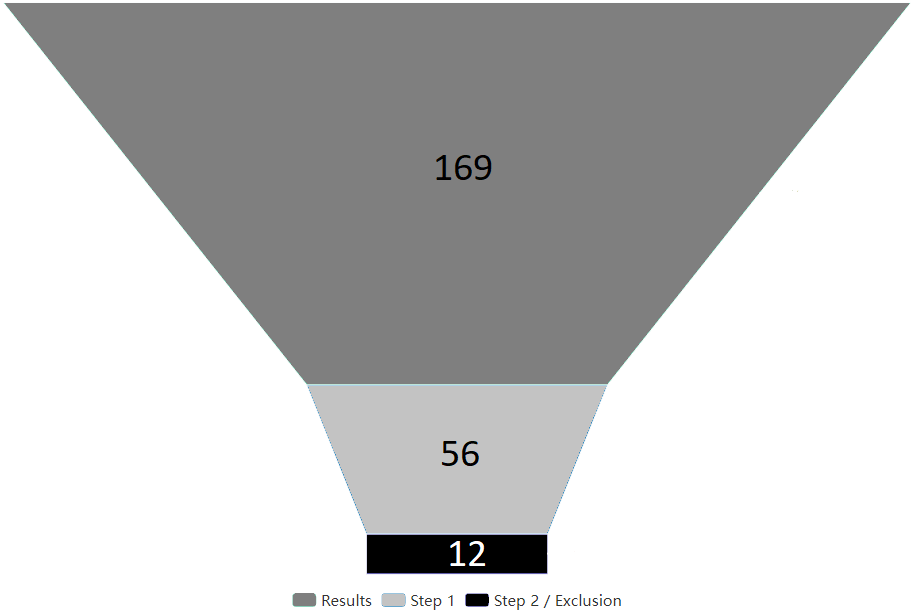
\includegraphics[width=12cm]{img/4-results.png}
  \end{center}
  \fonte{Author.}
\end{figure}

\subsection{Data Extraction}\label{sec:gl-data-extraction}

This section explains how the two data extractions from the discovered tools were carried out: one for the feature matrix and the other to collect more details on the key features shared by the tools.

\subsubsection{Feature Matrix}\label{sec:gl-feature-matrix}

It was important to develop a functions matrix among the filtered results after the research was completed in order to apply the quality standards. The authors were able to determine which features were present in the examined tools the most frequently in this method. There were determined to be 37 traits in total, some of which repeated more frequently than others. The matrix can be seen in \Cref{fig:gl-matrix}.

\begin{figure}[!htb]
  \caption{Feature Matrix}\label{fig:gl-matrix}
  \begin{center}
    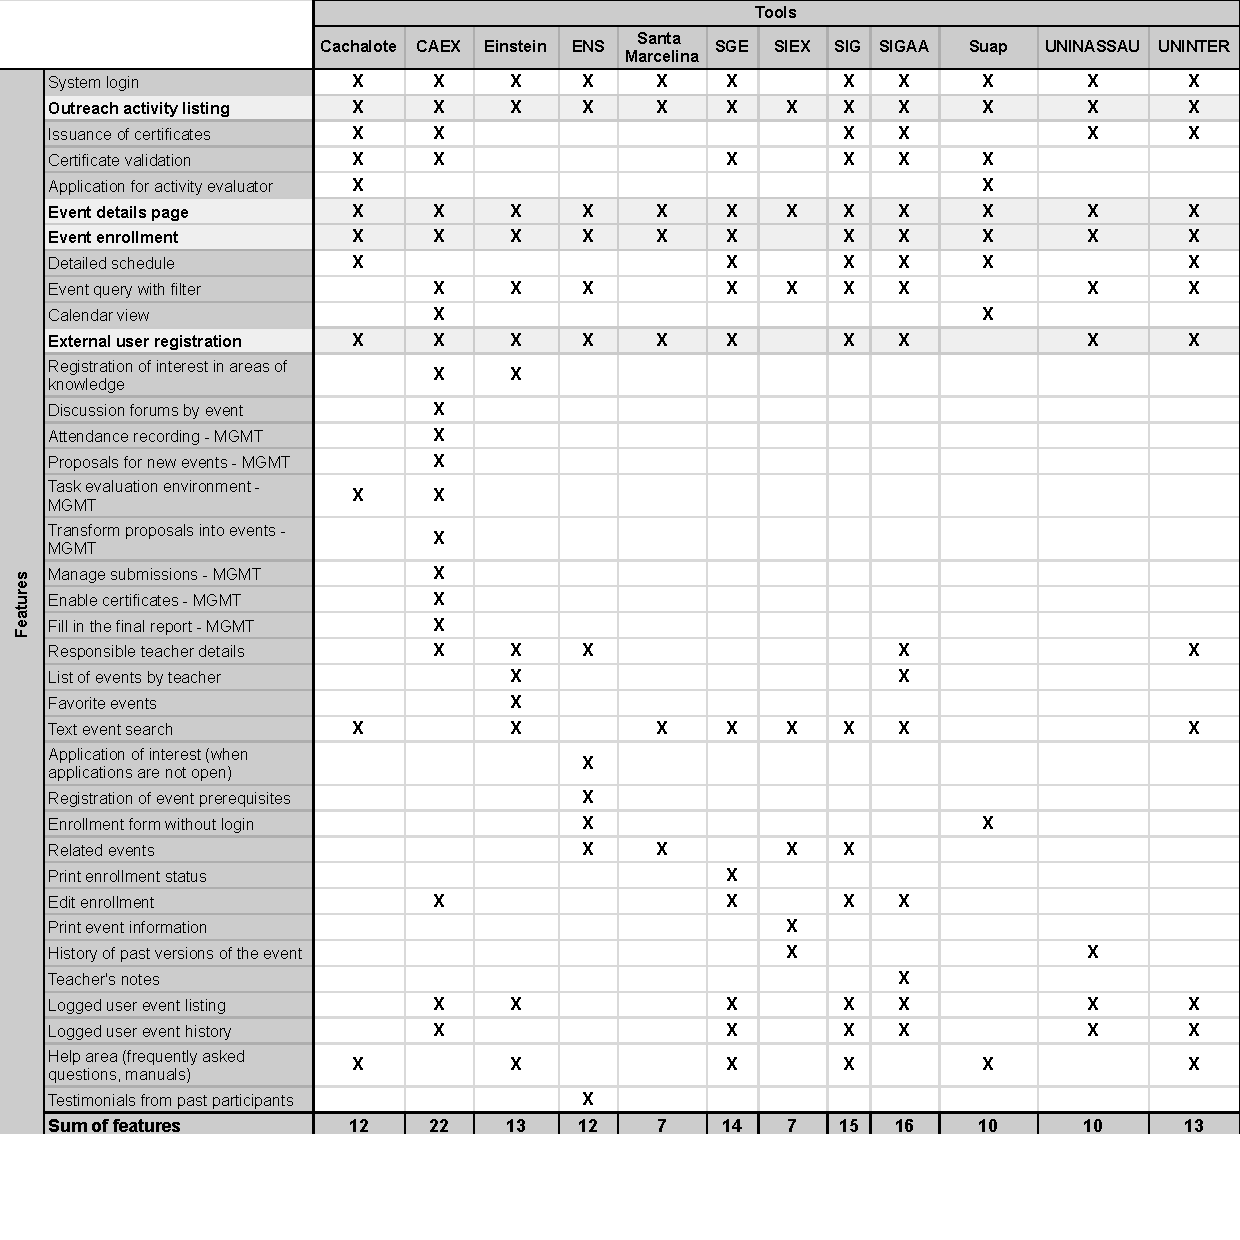
\includegraphics[width=16cm]{img/4-functionality-matrix.pdf}
  \end{center}
  \fonte{Author.}
\end{figure}

Lighter gray highlights were utilized to draw attention to the characteristics that were shared by all of the examined tools and websites so that they could be used as criteria in the subsequent stage of data extraction.

\subsubsection{More Information from Important Features}\label{sec:gl-data-extraction-2}

The goal of the second data extraction was to determine which data was utilized to 
\begin{inparaenum}[(i)]
  \item Listing of outreach activities;
  \item Detailed page of an activity;
  \item Enrollment of a participant into an activity;
  \item Registration of users external to the institution.
\end{inparaenum}

It was challenging to unify the analysis because each tool has its own format and attribute naming, thus the original names were retained. To prevent confusion, tools that lacked the chosen features have been highlighted in grey rather than having the cells left blank. Because it was nearly impossible to try to follow a pattern for all the tools, the extracted findings are written informally. The extracted data can be seen in \Cref{gl-additional-extraction}.

\begin{figure}[!htb]
  \caption{Additional Information Extraction}\label{fig:gl-additional-extraction}
  \begin{center}
    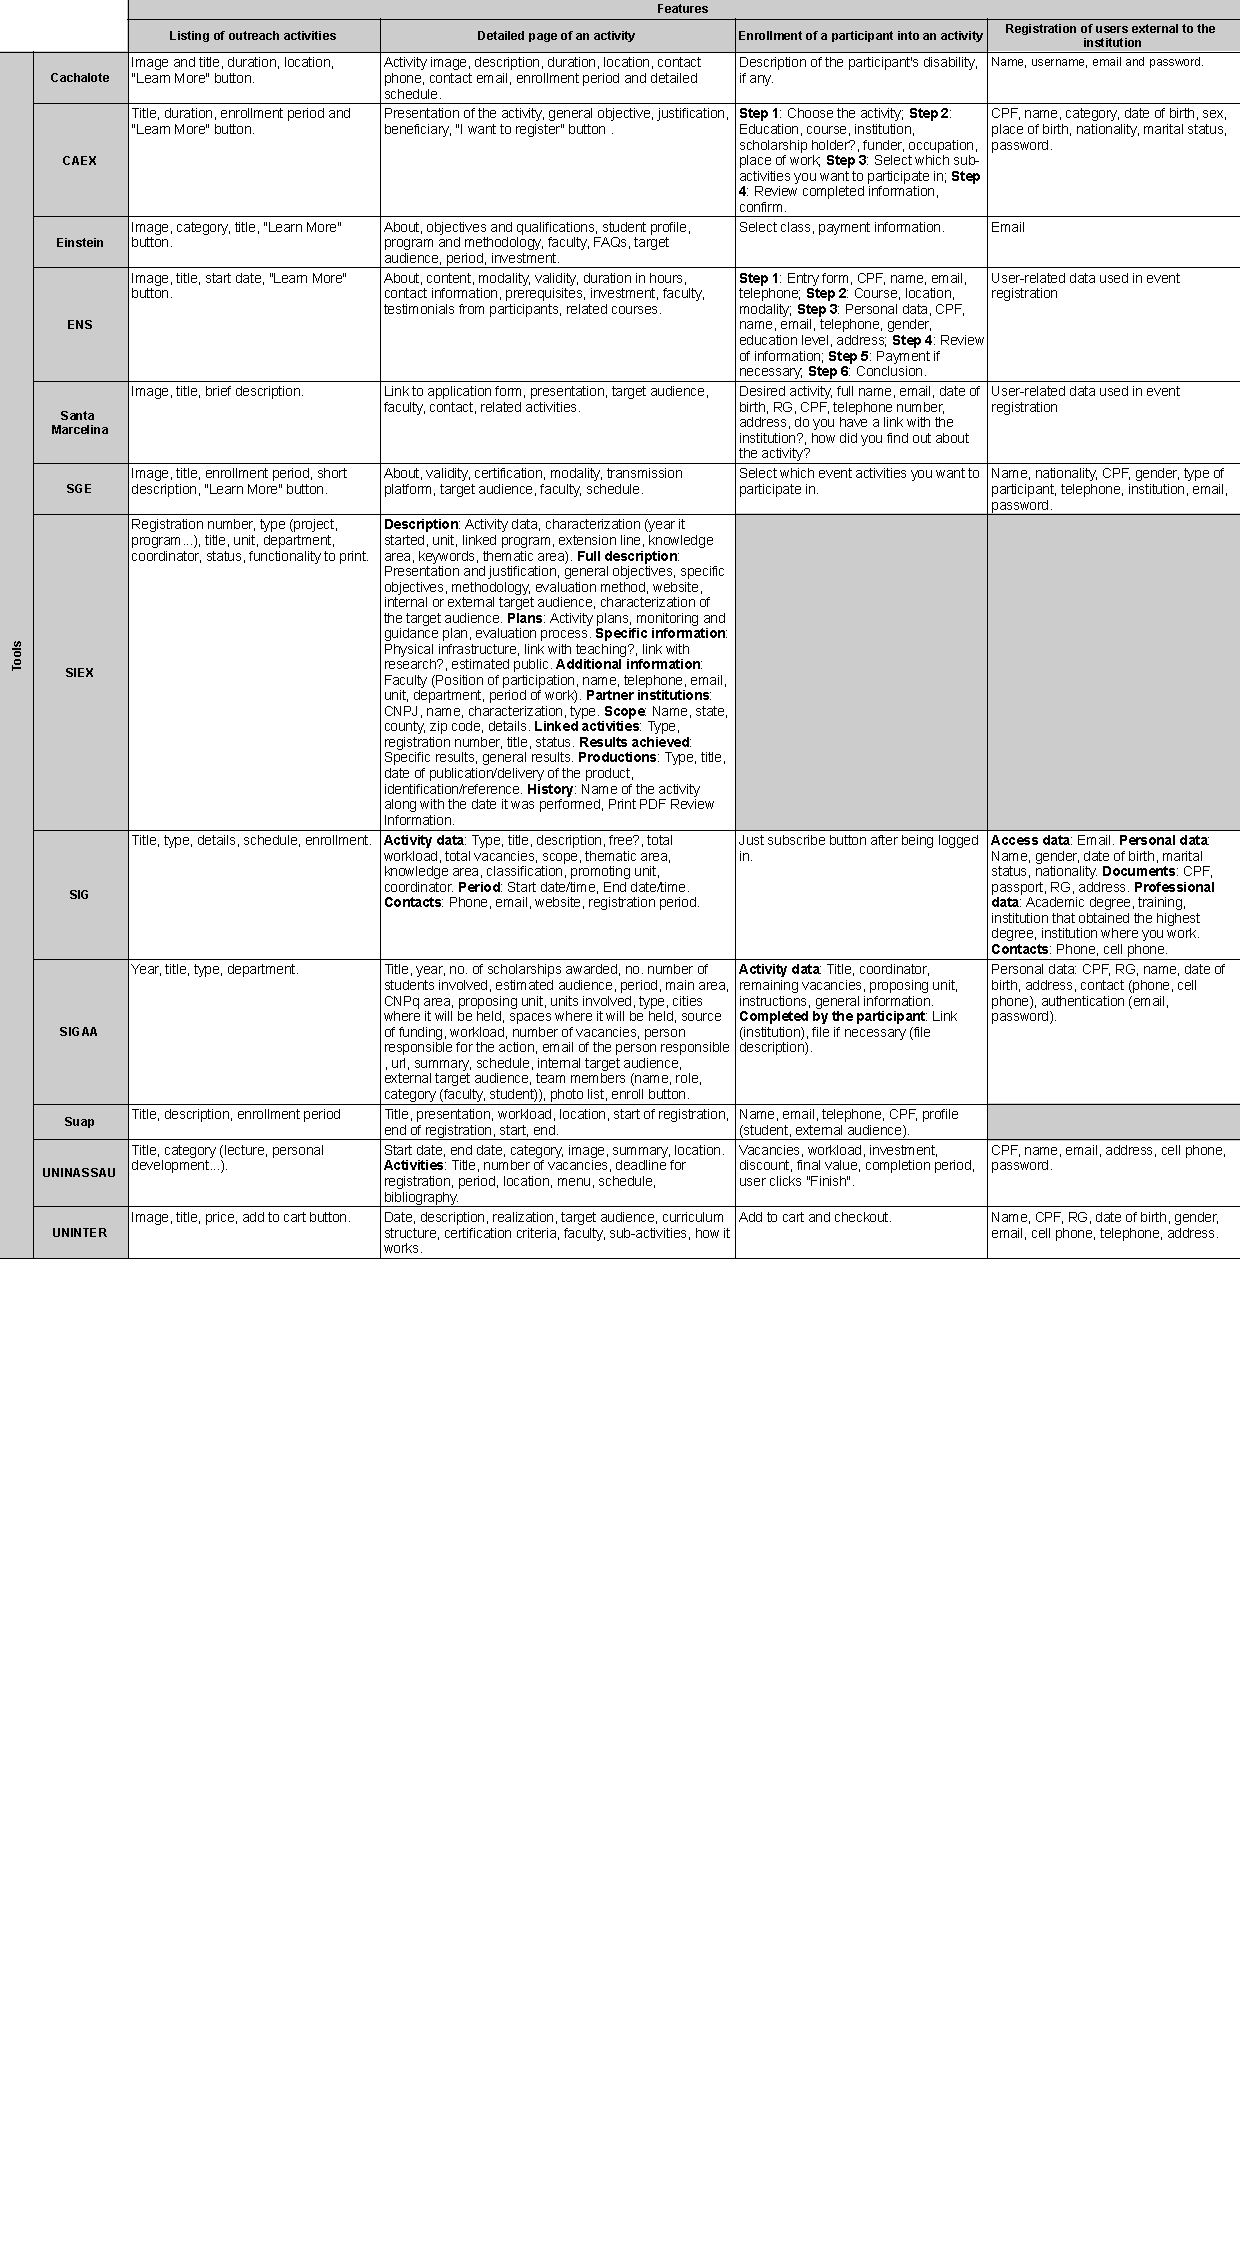
\includegraphics[width=16cm]{img/4-data-extraction-2.pdf}
  \end{center}
  \fonte{Author.}
\end{figure}

\subsection{Tool Classification}\label{sec:gl-tool-classification}

The extracted and tabulated data allowed for the classification of the tools based on the previously established quality standards. The scoring range for a tool is from 0 (zero) to 5 (five). The final results are shown in the table \Cref{tbl:gl-quality-criteria-results}.

\begin{table}[!htb]
  \centering
  \caption{Quality Criteria Evaluation}
  \label{tbl:gl-quality-criteria-results}
  \arrayrulecolor{black}
  \scriptsize
  \begin{tabular}{c|p{2cm}|cc|cc|cc|cc|cc|c}
    \hhline{~~-----------}
    \multicolumn{2}{l}{\multirow{3}{*}{~ ~ ~ ~ ~ ~}}                                & \multicolumn{11}{c}{{\cellcolor[rgb]{0.753,0.753,0.753}}\textbf{Quality Criteria ~ ~ ~ ~ ~ ~ ~ ~}}                                                                                                                                                                                                                                                                                                                                                                                                                                                                                                                                                                                                                                                                                                                                                         \\
    \hhline{~~-----------}
    \multicolumn{2}{l}{}                                                            & \multicolumn{2}{c|}{{\cellcolor[rgb]{0.753,0.753,0.753}}\textbf{QC 1. ~}}                          & \multicolumn{2}{c|}{{\cellcolor[rgb]{0.753,0.753,0.753}}\textbf{QC 2. ~}} & \multicolumn{2}{c|}{{\cellcolor[rgb]{0.753,0.753,0.753}}\textbf{QC 3. ~}} & \multicolumn{2}{c|}{{\cellcolor[rgb]{0.753,0.753,0.753}}\textbf{QC 4. ~}} & \multicolumn{2}{c|}{{\cellcolor[rgb]{0.753,0.753,0.753}}\textbf{QC 5. }} & \multicolumn{1}{l}{{\cellcolor[rgb]{0.753,0.753,0.753}}}                                                                                                                                                                                                                                                                                                                                                                               \\
    \multicolumn{2}{l}{}                                                            & {\cellcolor[rgb]{0.753,0.753,0.753}}\textbf{Ans.}                                                  & {\cellcolor[rgb]{0.753,0.753,0.753}}\textbf{Score}                        & {\cellcolor[rgb]{0.753,0.753,0.753}}\textbf{Ans.}                         & {\cellcolor[rgb]{0.753,0.753,0.753}}\textbf{Score}                        & {\cellcolor[rgb]{0.753,0.753,0.753}}\textbf{Ans.}                        & {\cellcolor[rgb]{0.753,0.753,0.753}}\textbf{Score}       & {\cellcolor[rgb]{0.753,0.753,0.753}}\textbf{Ans.} & {\cellcolor[rgb]{0.753,0.753,0.753}}\textbf{Score} & {\cellcolor[rgb]{0.753,0.753,0.753}}\textbf{Ans.} & {\cellcolor[rgb]{0.753,0.753,0.753}}\textbf{Score} & \multicolumn{1}{l}{\multirow{-2}{*}{{\cellcolor[rgb]{0.753,0.753,0.753}}\begin{tabular}[c]{@{}l@{}}\textbf{Final}\\\textbf{Results }\end{tabular}}}       \\
    \hhline{>{\arrayrulecolor[rgb]{0.753,0.753,0.753}}-->{\arrayrulecolor{black}}-----------}
    \rowcolor[rgb]{0.898,0.898,0.898} {\cellcolor[rgb]{0.753,0.753,0.753}}          & {\cellcolor[rgb]{0.753,0.753,0.753}}\textbf{Cachalote}                                             & 9                                                                         & 0,0                                                                       & No                                                                        & 0,0                                                                      & 12                                                       & 0,5                                               & Partially                                          & 0,5                                               & 2021                                               & 0,5                                                                                                                                                 & 1,5 \\
    {\cellcolor[rgb]{0.753,0.753,0.753}}                                            & {\cellcolor[rgb]{0.753,0.753,0.753}}\textbf{CAEX}                                                  & 4                                                                         & 0,0                                                                       & 7                                                                         & 1,0                                                                      & 22                                                       & 1,0                                               & Yes                                                & 1,0                                               & 2022                                               & 1,0                                                                                                                                                 & 4,0 \\
    \rowcolor[rgb]{0.898,0.898,0.898} {\cellcolor[rgb]{0.753,0.753,0.753}}          & {\cellcolor[rgb]{0.753,0.753,0.753}}\textbf{Einstein}                                              & 12                                                                        & 0,5                                                                       & 1                                                                         & 0,5                                                                      & 13                                                       & 0,5                                               & Partially                                          & 0,5                                               & 2022                                               & 1,0                                                                                                                                                 & 3,0 \\
    {\cellcolor[rgb]{0.753,0.753,0.753}}                                            & {\cellcolor[rgb]{0.753,0.753,0.753}}\textbf{ENS}                                                   & 11                                                                        & 0,5                                                                       & 3                                                                         & 1,0                                                                      & 12                                                       & 0,5                                               & Partially                                          & 0,5                                               & 2022                                               & 1,0                                                                                                                                                 & 3,5 \\
    \rowcolor[rgb]{0.898,0.898,0.898} {\cellcolor[rgb]{0.753,0.753,0.753}}          & {\cellcolor[rgb]{0.753,0.753,0.753}}\textbf{Santa Marcelina}                                       & 6                                                                         & 0,0                                                                       & No                                                                        & 0,0                                                                      & 7                                                        & 0,0                                               & Partially                                          & 0,5                                               & 2022                                               & 1,0                                                                                                                                                 & 1,5 \\
    {\cellcolor[rgb]{0.753,0.753,0.753}}                                            & {\cellcolor[rgb]{0.753,0.753,0.753}}\textbf{SGE}                                                   & 8                                                                         & 0,0                                                                       & 1                                                                         & 0,5                                                                      & 14                                                       & 1,0                                               & Yes                                                & 1,0                                               & 2016                                               & 0,0                                                                                                                                                 & 2,5 \\
    \rowcolor[rgb]{0.898,0.898,0.898} {\cellcolor[rgb]{0.753,0.753,0.753}}          & {\cellcolor[rgb]{0.753,0.753,0.753}}\textbf{SIEX}                                                  & 53                                                                        & 1,0                                                                       & 1                                                                         & 0,5                                                                      & 7                                                        & 0,0                                               & Yes                                                & 1,0                                               & 2022                                               & 1,0                                                                                                                                                 & 3,5 \\
    {\cellcolor[rgb]{0.753,0.753,0.753}}                                            & {\cellcolor[rgb]{0.753,0.753,0.753}}\textbf{SIG}                                                   & 18                                                                        & 0,5                                                                       & No                                                                        & 0,0                                                                      & 15                                                       & 1,0                                               & Partially                                          & 0,5                                               & 2022                                               & 1,0                                                                                                                                                 & 3,0 \\
    \rowcolor[rgb]{0.898,0.898,0.898} {\cellcolor[rgb]{0.753,0.753,0.753}}          & {\cellcolor[rgb]{0.753,0.753,0.753}}\textbf{SIGAA}                                                 & 28                                                                        & 1,0                                                                       & 1                                                                         & 0,5                                                                      & 16                                                       & 1,0                                               & Yes                                                & 1,0                                               & 2022                                               & 1,0                                                                                                                                                 & 4,5 \\
    {\cellcolor[rgb]{0.753,0.753,0.753}}                                            & {\cellcolor[rgb]{0.753,0.753,0.753}}\textbf{Suap}                                                  & 8                                                                         & 0,0                                                                       & No                                                                        & 0,0                                                                      & 10                                                       & 0,5                                               & Yes                                                & 1,0                                               & 2022                                               & 1,0                                                                                                                                                 & 2,5 \\
    \rowcolor[rgb]{0.898,0.898,0.898} {\cellcolor[rgb]{0.753,0.753,0.753}}          & {\cellcolor[rgb]{0.753,0.753,0.753}}\textbf{UNINASSAU}                                             & 14                                                                        & 0,5                                                                       & No                                                                        & 0,0                                                                      & 10                                                       & 0,5                                               & Partially                                          & 0,5                                               & 2022                                               & 1,0                                                                                                                                                 & 2,5 \\
    \multirow{-12}{*}{{\cellcolor[rgb]{0.753,0.753,0.753}}\rotcell{\textbf{Tools}}} & {\cellcolor[rgb]{0.753,0.753,0.753}}\textbf{UNINTER}                                               & 9                                                                         & 0,0                                                                       & No                                                                        & 0,0                                                                      & 13                                                       & 0,5                                               & Partially                                          & 0,5                                               & 2022                                               & 1,0                                                                                                                                                 & 2,0 \\
    \toprule
  \end{tabular}

  \fonte{Author.}
\end{table}

With this classification, it is clear that the \ac{CAEX} tool and \ac{SIGAA} received the highest ratings, which was exactly what was anticipated. First, \ac{SIGAA} is one of the academic management tools that institutions in the nation utilize the most, and \ac{CAEX} is the tool that offered the most distinctive features. As a result, they were two instruments that had a lot of promise and were very helpful in gathering data to create the goal product.

\subsection{Answering the Research Questions}\label{sec:gl-answer-research-questions}

The research questions are under the \Cref{tab:research-questions} and were introduced earlier in the study. For convenience's sake, each question is also explained below.

\begin{itemize}
  \item \textbf{RQ 1.} What tools currently exist that perform academic management?

        This is a question that also refers to some instruments that were eliminated during the use of inclusion and exclusion criteria. In this instance, 36 tools supporting academic management of various kinds were found, but only 12 of them meet the required requirements and are mentioned in the tool matrix in \Cref{fig:gl-matrix}.
  \item \textbf{RQ 1.1.} Which ones have related functionality or support outreach activities?

        The following tools were found, as it was already demonstrated in the \Cref{fig:gl-matrix}, which describes the relationships between tools and features:
        \begin{inparaenum}[(1)]
          \item Cachalote;
          \item CAEX;
          \item Einstein;
          \item ENS;
          \item Santa Marcelina;
          \item SGE;
          \item SIEX;
          \item SIG;
          \item SIGAA;
          \item SUAP;
          \item UNINASSAU and
          \item UNINTER.
        \end{inparaenum}

  \item \textbf{RQ 1.2.} What are the features offered by these tools?

        The features matrix, which is present in \Cref{fig:gl-matrix} and has a total of 37 features, contains a list of every feature that was discovered.
  \item \textbf{RQ 1.3.} What are the most common features between this type of tool?

        The most common functionalities in this type of tool are:
        \begin{inparaenum}[(i)]
          \item A login system;
          \item Lististing of \aclp{OA};
          \item \ac{OA} details page;
          \item \ac{OA} enrollment and
          \item Registration of external users.
        \end{inparaenum}
        The ability to search for events by text is another feature that is present regularly but not as frequently as the other features; 8 of the tools were found to support this functionality.
  \item \textbf{RQ 1.4.} What data do the tools use in relation to activities, participant registration and user registration?

        By analyzing the second data extraction presented in \Cref{sec:gl-data-extraction-2}, the most common fields for \acp{OA} are:
        \begin{inparaenum}[(a)]
          \item Title;
          \item Duration;
          \item Enrollment period;
          \item Contact information;
          \item Description;
          \item Target audience;
          \item Faculty and
          \item Schedule.
        \end{inparaenum}

        Regarding enrollment, the most common fields found are:
        \begin{inparaenum}[(a)]
          \item Participant's personal data;
          \item Institutional affiliation;
          \item Participant type and
          \item Information about the participant's disability, if any.
        \end{inparaenum}

        When it comes to user registration, these tools mostly employ personal information, authentication information, and an address; however, some also request information about the institution, participant type, and professional data.
\end{itemize}

\section{Validity}\label{sec:gl-validity}

Some validity threats were found as the systematic review mapping process progressed. While the writers were able to lessen the majority of them, some still need to be addressed. They are as follows:

\begin{itemize}
  \item When comparing the findings they both found throughout the study phase, the authors observed that the search results varied just little, between one or two different records. Although it was a hazard that could be easily reduced, it couldn't be fully ruled out. In order to do the search in anonymous mode, the approach employed was to log out of the account currently logged into the browser. As a result, there were fewer divergences overall, however occasionally divergent outcomes did occur.
  \item Functionalities of the tools weren't checked with the creators. Unfortunately, the authors were unable to reach any universities to inquire about the management solution being employed.
  \item The authors aimed to conduct the search in as little time as feasible, beginning and finishing it in just three days, in order to reduce the divergence of findings. As the search engine is regarded as a ``black box'', making it challenging to predict the precise results that will emerge with each search string, the longer the delay, the greater the chance that risks to the study will be introduced.
\end{itemize}

\section{Considerations}\label{sec:gl-considerations}

Finding tools that are similar to the intended outcome of the entire study was made possible by this thorough review of the grey literature. Before undertaking the review, no knowledge of the current status of the field or the most popular solutions employed by Brazilian \ac{HEI} existed.

A wealth of useful data was gathered regarding the instruments used today. It was now much more obvious what \aclp{OA} management and processes covered. This information will be useful when putting the objective product into use, which seeks to provide a comprehensive solution for \ac{OA} management.

Furthermore, the review protocol's definitions of all the research questions could all be answered.